\documentclass[11pt,]{article}
\usepackage[margin=1in]{geometry}
\newcommand*{\authorfont}{\fontfamily{phv}\selectfont}
\usepackage[]{mathpazo}

\usepackage{amssymb,amsmath}
\usepackage{xcolor}

%TIKZ and Flow chart material
\usepackage{tikz}
\usetikzlibrary{shapes.geometric, arrows}
\tikzstyle{startstop} = [rectangle, rounded corners, minimum width=3cm, minimum height=1cm,text centered, draw=black, fill=red!30]
\tikzstyle{io} = [trapezium, trapezium left angle=70, trapezium right angle=110, minimum width=3cm, minimum height=1cm, text centered, draw=black,fill=white]
\tikzstyle{process} = [rectangle, minimum width=3cm, minimum height=1cm, text centered, draw=black, fill=white]
\tikzstyle{decision} = [diamond, minimum width=3cm, minimum height=1cm, text centered, draw=black, fill=white]
\tikzstyle{smalldecision} = [diamond, minimum width=1cm, minimum height=1cm, text centered, draw=black, fill=white]
\tikzstyle{arrow} = [thick,->,>=stealth]
\tikzstyle{line} = [thick,-]
\tikzstyle{dot} = [circle,inner sep=0.5pt,draw=black, fill=black]


%\tikzstyle{startstop} = [rectangle, rounded corners, minimum width=3cm, minimum height=1cm,text centered, %draw=black, fill=red!30]
%\tikzstyle{io} = [trapezium, trapezium left angle=70, trapezium right angle=110, minimum width=3cm, %minimum height=1cm, text centered, draw=black,fill=white]
%\tikzstyle{process} = [rectangle, minimum width=3cm, minimum height=1cm, text centered, draw=black, %fill=white]
%\tikzstyle{decision} = [diamond, minimum width=3cm, minimum height=1cm, text centered, draw=black, %fill=green!30]
%\tikzstyle{arrow} = [thick,->,>=stealth]




\usepackage{abstract}
\renewcommand{\abstractname}{}    % clear the title
\renewcommand{\absnamepos}{empty} % originally center
\newcommand{\blankline}{\quad\pagebreak[2]}

\providecommand{\tightlist}{%
  \setlength{\itemsep}{0pt}\setlength{\parskip}{0pt}}
\usepackage{longtable,booktabs}

\usepackage{parskip}
\usepackage{titlesec}
\titlespacing\section{0pt}{12pt plus 4pt minus 2pt}{6pt plus 2pt minus 2pt}
\titlespacing\subsection{0pt}{12pt plus 4pt minus 2pt}{6pt plus 2pt minus 2pt}

\titleformat*{\subsubsection}{\normalsize\itshape}

\usepackage{titling}
\setlength{\droptitle}{-.25cm}

%\setlength{\parindent}{0pt}
%\setlength{\parskip}{6pt plus 2pt minus 1pt}
%\setlength{\emergencystretch}{3em}  % prevent overfull lines

\usepackage[T1]{fontenc}
\usepackage[utf8]{inputenc}

\usepackage{fancyhdr}
\pagestyle{fancy}
\usepackage{lastpage}
\renewcommand{\headrulewidth}{0.3pt}
\renewcommand{\footrulewidth}{0.0pt}
%\lhead{\footnotesize Pre-exam problem Set }
\lhead{\footnotesize BUEC 311: Pre-exam problem Set, Game Theory and
Government Intervention}
\rhead{\footnotesize \today}
\lfoot{\small \copyright }
\cfoot{}
\rfoot{\small \thepage/\pageref*{LastPage}}

\fancypagestyle{firststyle}
{
\renewcommand{\headrulewidth}{0pt}%
   \fancyhf{}
   \fancyfoot[C]{\thepage/\pageref*{LastPage}}
}

%\def\labelitemi{--}
%\usepackage{enumitem}
%\setitemize[0]{leftmargin=25pt}
%\setenumerate[0]{leftmargin=25pt}




\makeatletter
\@ifpackageloaded{hyperref}{}{%
\ifxetex
  \usepackage[setpagesize=false, % page size defined by xetex
              unicode=false, % unicode breaks when used with xetex
              xetex]{hyperref}
\else
  \usepackage[unicode=true]{hyperref}
\fi
}
\@ifpackageloaded{color}{
    \PassOptionsToPackage{usenames,dvipsnames}{color}
}{%
    \usepackage[usenames,dvipsnames]{color}
}
\makeatother
\hypersetup{breaklinks=true,
            bookmarks=true,
            pdfauthor={},
             pdfkeywords = {},
            pdftitle={Pre-exam problem Set: Game Theory and Government
Intervention},
            colorlinks=true,
            citecolor=blue,
            urlcolor=blue,
            linkcolor=magenta,
            pdfborder={0 0 0}}
\urlstyle{same}  % don't use monospace font for urls


\setcounter{secnumdepth}{0}


%%\usepackage{graphicx}
% We will generate all images so they have a width \maxwidth. This means
% that they will get their normal width if they fit onto the page, but
% are scaled down if they would overflow the margins.
%\makeatletter
%\def\maxwidth{\ifdim\Gin@nat@width>\linewidth\linewidth
%\else\Gin@nat@width\fi}
%\makeatother
%\let\Oldincludegraphics\includegraphics
%\renewcommand{\includegraphics}[1]{\Oldincludegraphics[width=\maxwidth]{#1}}
%



\usepackage{setspace}

\title{\vspace{-1.5cm}\Large{BUEC 311: Business Economics, Organization
and Management}\medskip\\\Large{Pre-exam problem Set}
\medskip\\\Large{Game Theory and Government Intervention}
}
\date{\vspace{-.75cm}\Large{\today}}

\definecolor{light-gray}{gray}{0.8}


\begin{document}

\vspace{-5cm}\maketitle
 \tikz [remember picture,overlay]
    %\node[yshift=-1.65cm,xshift=0cm] at (current page.north)
    %\node[yshift=-1.65cm,xshift=0cm] at (current page.north)
        %or: (current page.center)
        \node[yshift=-1cm,xshift=6.5cm] at (current page.north west)
        %{
\includegraphics[width=3in]{UA-ASB-COLOUR.png}};
        {
\includegraphics[width=.5\paperwidth]{../images/UA-ASB-COLOUR.png}};
\vspace{-.75cm}		
		\thispagestyle{firststyle}



\begin{enumerate}
\def\labelenumi{\arabic{enumi})}
\tightlist
\item
  Market failures \_\_\_\_\_\_\_\_ and generate \_\_\_\_\_\_\_\_.
\end{enumerate}

\begin{enumerate}
\def\labelenumi{\Alph{enumi})}
\tightlist
\item
  force governments to act; regulations
\item
  create monopolies or oligopolies; deadweight loss
\item
  reduce economic efficiency; deadweight loss
\item
  create deadweight loss; externalities Answer: C
\end{enumerate}

\begin{enumerate}
\def\labelenumi{\arabic{enumi})}
\setcounter{enumi}{1}
\tightlist
\item
  Which of the following is a dynamic game?
\end{enumerate}

\begin{enumerate}
\def\labelenumi{\Alph{enumi})}
\tightlist
\item
  Rock-paper-scissors
\item
  Craps (bet on a roll of the dice)
\item
  Chess
\item
  Rock-paper-scissors-lizard-Spock Answer: C
\end{enumerate}

\begin{enumerate}
\def\labelenumi{\arabic{enumi})}
\setcounter{enumi}{2}
\tightlist
\item
  In a repeated prisoners' dilemma type game where the static Nash
  equilibrium is worse than collaboration for both players
\end{enumerate}

\begin{enumerate}
\def\labelenumi{\Alph{enumi})}
\tightlist
\item
  the players act sequentially.
\item
  the outcomes are the same as in a static prisoners' dilemma game.
\item
  firms' choices are not influenced by their opponents' actions.
\item
  cooperation may result if the game is played indefinitely. Answer: D
\end{enumerate}

\begin{enumerate}
\def\labelenumi{\arabic{enumi})}
\setcounter{enumi}{3}
\tightlist
\item
  In an indefinitely repeated game, a firm might use a \_\_\_\_\_\_\_\_
  to \_\_\_\_\_\_\_\_ a rival that defects from a cooperative strategy.
\end{enumerate}

\begin{enumerate}
\def\labelenumi{\Alph{enumi})}
\tightlist
\item
  trigger strategy; threaten
\item
  trigger strategy; punish
\item
  legal maneuver; sue
\item
  tacit threat; dissuade Answer: B
\end{enumerate}

\begin{enumerate}
\def\labelenumi{\arabic{enumi})}
\setcounter{enumi}{4}
\tightlist
\item
  If firms adopt a strategy that triggers a permanent punishment in a
  prisoner's dilemma game (the United vs American Airlines game we did
  in class, for example), the result in an indefinitely repeated game is
\end{enumerate}

\begin{enumerate}
\def\labelenumi{\Alph{enumi})}
\tightlist
\item
  undefined.
\item
  the noncooperative Nash equilibrium.
\item
  the collusive Nash equilibrium.
\item
  economically inefficient. Answer: C
\end{enumerate}

\newpage

\begin{enumerate}
\def\labelenumi{\arabic{enumi})}
\setcounter{enumi}{5}
\tightlist
\item
  A model of oligopoly in which one firm moves first, and then the other
  rivals follow is a \_\_\_\_\_\_\_\_ game.
\end{enumerate}

\begin{enumerate}
\def\labelenumi{\Alph{enumi})}
\tightlist
\item
  Stackelberg model
\item
  Cournot model
\item
  finite move
\item
  tit-for-tat Answer: A
\end{enumerate}

\begin{enumerate}
\def\labelenumi{\arabic{enumi})}
\setcounter{enumi}{6}
\tightlist
\item
  The Cournot and Stackelberg models are similar, EXCEPT Cournot
  \_\_\_\_\_\_\_\_ and Stackelberg \_\_\_\_\_\_\_\_.
\end{enumerate}

\begin{enumerate}
\def\labelenumi{\Alph{enumi})}
\tightlist
\item
  sets price; sets output
\item
  sets output; sets price
\item
  is dynamic; is static
\item
  is static; is dynamic Answer: D
\end{enumerate}

\begin{enumerate}
\def\labelenumi{\arabic{enumi})}
\setcounter{enumi}{7}
\tightlist
\item
  Which of the following statements is TRUE?
\end{enumerate}

\begin{enumerate}
\def\labelenumi{\Alph{enumi})}
\tightlist
\item
  A government policy that eliminates a market failure, but only some
  people gain while others are kept the same, is not a Pareto
  improvement.
\item
  A government policy that eliminates a market failure, but only some
  people gain while others are kept the same, is a Pareto improvement.
\item
  A government policy that eliminates a market failure and some people
  gain and some lose only a little, is a Pareto improvement.
\item
  A government policy that generates a Pareto improvement eliminates all
  deadweight loss. Answer: B
\end{enumerate}

\begin{enumerate}
\def\labelenumi{\arabic{enumi})}
\setcounter{enumi}{8}
\tightlist
\item
  Governments can eliminate market failure due to an imperfectly
  competitive market by
\end{enumerate}

\begin{enumerate}
\def\labelenumi{\Alph{enumi})}
\tightlist
\item
  changing the market structure, for example by eliminating monopoly
  protection.
\item
  having the government own the monopoly.
\item
  imposing regulations that reduce prices.
\item
  All of the above. Answer: D
\end{enumerate}

\begin{enumerate}
\def\labelenumi{\arabic{enumi})}
\setcounter{enumi}{9}
\tightlist
\item
  Optimal price regulation sets price equal to
\end{enumerate}

\begin{enumerate}
\def\labelenumi{\Alph{enumi})}
\tightlist
\item
  marginal cost.
\item
  average variable cost.
\item
  average cost.
\item
  minimum average cost. Answer: A
\end{enumerate}

\begin{enumerate}
\def\labelenumi{\arabic{enumi})}
\setcounter{enumi}{10}
\tightlist
\item
  In order to regulate a monopoly's price, the government
\end{enumerate}

\begin{enumerate}
\def\labelenumi{\Alph{enumi})}
\tightlist
\item
  needs to hire former executives from the monopoly.
\item
  should rely on industry experts for information.
\item
  needs accurate information on the monopoly's demand and cost curves.
\item
  needs to know the monopoly's supply curve. Answer: C
\end{enumerate}

\begin{enumerate}
\def\labelenumi{\arabic{enumi})}
\setcounter{enumi}{11}
\tightlist
\item
  Government regulation in the market
\end{enumerate}

\begin{enumerate}
\def\labelenumi{\Alph{enumi})}
\tightlist
\item
  always increases consumer surplus.
\item
  always passes the cost-benefit test.
\item
  always solves market failures.
\item
  None of the above. Answer: D \newpage
\end{enumerate}

\begin{enumerate}
\def\labelenumi{\arabic{enumi})}
\setcounter{enumi}{12}
\tightlist
\item
  Regulation might NOT increase total surplus because
\end{enumerate}

\begin{enumerate}
\def\labelenumi{\Alph{enumi})}
\tightlist
\item
  the costs of the regulation might outweigh the benefits.
\item
  it may not be possible to gather the information necessary to set
  prices correctly.
\item
  regulators might get captured or influenced by the industry and set
  policies to benefit producers over consumers.
\item
  All of the above. Answer: D
\end{enumerate}

\begin{enumerate}
\def\labelenumi{\arabic{enumi})}
\setcounter{enumi}{13}
\tightlist
\item
  In general, an externality is created when
\end{enumerate}

\begin{enumerate}
\def\labelenumi{\Alph{enumi})}
\tightlist
\item
  people are affected (other than by changes in market prices) by a
  transaction which they were not part of.
\item
  firms produce a product of low quality and consumers don't like it.
\item
  firms have to pay for pollution the environment.
\item
  the government subsidizes education.
\item
  David Suzuki says so. Answer: A
\end{enumerate}

\begin{enumerate}
\def\labelenumi{\arabic{enumi})}
\setcounter{enumi}{14}
\tightlist
\item
  Students who talk loudly with each other in class
\end{enumerate}

\begin{enumerate}
\def\labelenumi{\Alph{enumi})}
\tightlist
\item
  create an externality because other students cannot follow the lecture
  as well.
\item
  disturb nobody.
\item
  benefit the other students in class because they engage in
  conversation.
\item
  only create an externality if they talk about something unrelated to
  class. Answer: A
\end{enumerate}

\begin{enumerate}
\def\labelenumi{\arabic{enumi})}
\setcounter{enumi}{15}
\tightlist
\item
  A game includes
\end{enumerate}

\begin{enumerate}
\def\labelenumi{\Alph{enumi})}
\tightlist
\item
  a strategy.
\item
  payoffs.
\item
  rules.
\item
  All of the above. Answer: D
\end{enumerate}

\begin{enumerate}
\def\labelenumi{\arabic{enumi})}
\setcounter{enumi}{16}
\tightlist
\item
  A strategy is dominant if
\end{enumerate}

\begin{enumerate}
\def\labelenumi{\Alph{enumi})}
\tightlist
\item
  it yields a greater payoff than any other player receives.
\item
  it yields a payoff at least as large as that from any other strategy,
  regardless of the actions of other players.
\item
  the player cannot gain by changing strategy, assuming that no other
  player changes strategy.
\item
  it is part of a Nash equilibrium. Answer: B
\end{enumerate}

\begin{enumerate}
\def\labelenumi{\arabic{enumi})}
\setcounter{enumi}{17}
\tightlist
\item
  One interesting feature of a prisoner's dilemma game (the United vs
  American Airlines game we did in class, for example) is that
\end{enumerate}

\begin{enumerate}
\def\labelenumi{\Alph{enumi})}
\tightlist
\item
  non-cooperative behavior leads to lower payoffs than cooperative
  behavior.
\item
  there is never a dominated strategy.
\item
  individuals behave irrationally when they behave non-cooperatively.
\item
  cooperative behavior leads to lower payoffs than non-cooperative
  behavior. Answer: A
\end{enumerate}

\begin{enumerate}
\def\labelenumi{\arabic{enumi})}
\setcounter{enumi}{18}
\tightlist
\item
  An auction in which the price announced by the auctioneer DESCENDS is
  called a(n)
\end{enumerate}

\begin{enumerate}
\def\labelenumi{\Alph{enumi})}
\tightlist
\item
  Dutch Auction.
\item
  English Auction.
\item
  Sealed Bid Auction.
\item
  Descending Option Auction. Answer: A
\end{enumerate}

\begin{enumerate}
\def\labelenumi{\arabic{enumi})}
\setcounter{enumi}{19}
\tightlist
\item
  Assuming individuals follow their optimal bidding strategies, the
  individual with the highest valuation of the good will win in which of
  the following auctions?
\end{enumerate}

\begin{enumerate}
\def\labelenumi{\Alph{enumi})}
\tightlist
\item
  English Auction
\item
  Dutch Auction
\item
  First-price Sealed Bid Auction
\item
  Second-price Sealed Bid Auction
\item
  All of the above. Answer: E
\end{enumerate}

\begin{enumerate}
\def\labelenumi{\arabic{enumi})}
\setcounter{enumi}{20}
\tightlist
\item
  In a second-price auction, the winner pays
\end{enumerate}

\begin{enumerate}
\def\labelenumi{\Alph{enumi})}
\tightlist
\item
  the second-to-last bid it made.
\item
  the average of the top two bids.
\item
  the amount bid by the runner-up.
\item
  None of the above. Answer: C
\end{enumerate}

\begin{enumerate}
\def\labelenumi{\arabic{enumi})}
\setcounter{enumi}{21}
\tightlist
\item
  The winner's curse occurs when
\end{enumerate}

\begin{enumerate}
\def\labelenumi{\Alph{enumi})}
\tightlist
\item
  bidders ``shade'' their bids.
\item
  the winning bid is higher than the good's common value.
\item
  the winner buys something he didn't need.
\item
  the winning bid is higher than the private value of the good. Answer:
  B
\end{enumerate}

\begin{enumerate}
\def\labelenumi{\arabic{enumi})}
\setcounter{enumi}{22}
\tightlist
\item
  It is unwise to bid more than your valuation of the good in a sealed
  bid second-price auction because
\end{enumerate}

\begin{enumerate}
\def\labelenumi{\Alph{enumi})}
\tightlist
\item
  you will have to pay more than twice your valuation
\item
  you want to make sure you don't win
\item
  you might end up winning and paying more than the item is worth to you
\item
  you don't know what a second price auction is Answer: C
\end{enumerate}

\begin{enumerate}
\def\labelenumi{\arabic{enumi})}
\setcounter{enumi}{23}
\tightlist
\item
  Repeated games are conducive to
\end{enumerate}

\begin{enumerate}
\def\labelenumi{\Alph{enumi})}
\tightlist
\item
  explicit cooperation or collusion.
\item
  tacit cooperation or collusion.
\item
  corruption.
\item
  failing to have a Nash equilibrium. Answer: B
\end{enumerate}

\begin{enumerate}
\def\labelenumi{\arabic{enumi})}
\setcounter{enumi}{24}
\tightlist
\item
  In rock-paper-scissors, which of the following is a pure strategy Nash
  equilibrium:
\end{enumerate}

\begin{enumerate}
\def\labelenumi{\Alph{enumi})}
\tightlist
\item
  playing rock, because nothing beats rock
\item
  playing scissors, because most people play paper
\item
  playing paper, because your opponent likely thinks nothing beats rock
\item
  none of the above
\end{enumerate}

Answer: D

\begin{enumerate}
\def\labelenumi{\arabic{enumi})}
\setcounter{enumi}{24}
\tightlist
\item
  In rock-paper-scissors-lizard-Spock (see next page), which of the
  following is a pure strategy Nash equilibrium:
\end{enumerate}

\begin{figure}
\centering
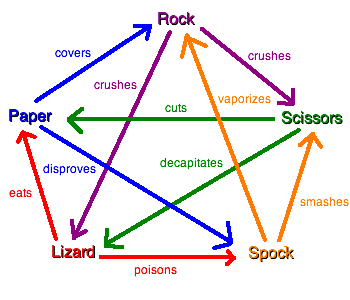
\includegraphics{Rock_paper_scissors_lizard_spock.png}
\caption{Rock-Paper-Scissors-Lizard-Spock}
\end{figure}

\begin{enumerate}
\def\labelenumi{\Alph{enumi})}
\tightlist
\item
  playing rock, because nothing beats rock
\item
  playing scissors, because most people play paper
\item
  playing paper, because your opponent likely thinks nothing beats rock
\item
  Logically, it has to be Spock.
\item
  None of the above
\end{enumerate}

Answer: E




\end{document}
